%----------------------------------------------------------------------------
%
%	This template was created by
%		Christian Krieg <christian.krieg@alumni.tuwien.ac.at>
%
%	April 2018
%
%----------------------------------------------------------------------------
%
\documentclass[%
	a4paper,
]
{article}
%
%----------------------------------------------------------------------------
%
% Institution
%
%\institution{Institute of Computer Technology}
%
%----------------------------------------------------------------------------
%
% Use the 'Libertine' font type
%
\usepackage{libertine}
\usepackage[T1]{fontenc}
\usepackage[utf8]{inputenc}
%
%----------------------------------------------------------------------------
%
% Set page margins
%
\usepackage{geometry}
\geometry{%
	left   = 2cm,
	right  = 2cm,
	top    = 2cm,
	bottom = 2cm
}
%
%----------------------------------------------------------------------------
%
% Set line spacing
%
\usepackage{setspace}
\setstretch{1}
%
%----------------------------------------------------------------------------
%
% Set paragraph: No indentation, but include an empty line
%
\usepackage[parfill]{parskip}
%
%----------------------------------------------------------------------------
%
% Settings for hyperlinks
%
\usepackage{hyperref}
\hypersetup{%
	colorlinks = true,
	allcolors  = blue,
}
%
%----------------------------------------------------------------------------
%
% Use colors
%
\usepackage{xcolor}
\usepackage{colortbl}
%
%----------------------------------------------------------------------------
%
% Define a TODO and a DONE command
%
\newcommand{\todo}[1]{\textcolor{red}{#1}}
\newcommand{\done}[1]{}
%
%----------------------------------------------------------------------------
%
% Use glossaries
%
\usepackage{glossaries}
\makeglossaries
%
% Glossary entries
%
\newglossaryentry{fpga}{
	name = {FPGA},
	description = {Field-programmable gate array},
	text = {FPGA},
	first = {field-programmable gate array (FPGA)},
	plural = {FPGAs},
	firstplural = {field-programmable gate arrays (FPGAs)},
}
%
\newglossaryentry{trng}{
	name = {TRNG},
	description = {True-random number generator},
	text = {TRNG},
	first = {true-random number generator (TRNG)},
	plural = {TRNGs},
	firstplural = {true-random number generators (TRNGs)},
}
%
\newglossaryentry{bcd}{
  name={BCD},
  description={Binary-coded decimal},
  text={BCD},
  first={binary-coded decimal (BCD)},
}
%
\newglossaryentry{hdl}{
  name={HDL},
  description={Hardware description language},
  text={HDL},
  first={hardware description language (HDL)},
  plural={HDLs},
  firstplural={hardware description languages (HDLs)},
}
%
\newglossaryentry{ip}{
  name={IP},
  description={Intellectual property},
  text={IP},
  first={intellectual property (IP)},
}
%
\newglossaryentry{3pip}{
  name={3PIP},
  description={Third-party intellectual property},
  text={3PIP},
  first={third-party intellectual property (3PIP)},
}
%
\newglossaryentry{dsp}{
  name={DSP},
  description={Digital signal processor},
  text={DSP},
  first={digital signal processor (DSP)},
  plural={DSPs},
  firstplural={digital signal processors (DSPs)},
}
%
\newglossaryentry{amba}{
  name={AMBA},
  description={Advanced microcontroller bus architecture},
  text={AMBA},
  first={advanced microcontroller bus architecture (AMBA)},
}
%
\newglossaryentry{apb}{
  name={APB},
  description={Advanced peripheral bus},
  text={APB},
  first={advanced peripheral bus (APB)},
}
%
%\newglossaryentry{}{
%  name={},
%  description={},
%  text={},
%  first={},
%  plural={},
%  firstplural={},
%}
%
%----------------------------------------------------------------------------
%
% Using URLs
%
\usepackage{url}
%
%
%% Define a new style with a smaller font.
\makeatletter
\def\url@footnotestyle{%
  \@ifundefined{selectfont}{\def\UrlFont{\sf}}{\def\UrlFont{\footnotesize\rmfamily}}}
\makeatother
%% Now actually use the newly defined style.
\urlstyle{footnote}
%
%
%
%% Define a new style with a larger font.
\makeatletter
\def\url@normalstyle{%
  \@ifundefined{selectfont}{\def\UrlFont{\sf}}{\def\UrlFont{\normalsize\rmfamily}}}
\makeatother
%% Now actually use the newly defined style.
\urlstyle{footnote}
%
%----------------------------------------------------------------------------
%
% Settings for citations and the bibliography
%
\usepackage[%
	backend     = biber,
	maxbibnames = 99,
	autocite    = footnote,
	citestyle   = verbose-ibid,
	firstinits=true,
]{biblatex}
\bibliography{bib/task-2}
%
%----------------------------------------------------------------------------
%
%	TikZ -- TikZ ist kein Zeichenprogramm
%
\usepackage{tikz}
\usepackage{tikz-timing}
\usepackage{etoolbox}
\usetikzlibrary{mindmap}
\usetikzlibrary{shapes}
\usetikzlibrary{arrows}
\usetikzlibrary{decorations}
\usetikzlibrary{shapes.symbols}
\usetikzlibrary{shapes.geometric}
\usetikzlibrary{shapes.multipart}
\usetikzlibrary{positioning}
\usetikzlibrary{patterns}
\usetikzlibrary{calc}
\usetikzlibrary{scopes}         % cf. pgfmanual p.66
\usetikzlibrary{chains}         % cf. pgfmanual p.284
\usetikzlibrary{fit}
\usetikzlibrary{matrix}
\usetikzlibrary{decorations}
\usetikzlibrary{circuits.logic}
\usetikzlibrary{circuits.logic.IEC}
\usetikzlibrary{shapes.gates.logic.IEC}
\usetikzlibrary{circuits.logic.US}
\usetikzlibrary{shapes.gates.logic.US}
\usetikzlibrary{circuits.ee}
\usetikzlibrary{circuits.ee.IEC}
\usetikzlibrary{backgrounds}
\usetikzlibrary{automata}
\usetikzlibrary{intersections}
\usetikzlibrary{plotmarks}
\usepgflibrary{fpu}
\usetikzlibrary{decorations.pathreplacing}
%
%----------------------------------------------------------------------------
%
% TikZ shapes
%  
	% D flip-flops (DFFs) and shift register
% Author: Martin Scharrer
%\documentclass[a4paper,landscape]{article}

%\usepackage{pgf,tikz}
%%%<
%\usepackage{verbatim}
%\usepackage[active,tightpage]{preview}
%\PreviewEnvironment{tikzpicture}
%\setlength\PreviewBorder{5pt}%
%%%>

%\begin{comment}
%:Title: D flip-flops and shift register
%
%Example of a custom node shape for drawing  D flip-flops. The shape is used to draw a serial shift
%register. 
%
%\end{comment}
%
%\usetikzlibrary{calc,arrows}
%\usepackage{amsmath}
%\usepackage[left=1cm,right=1cm]{geometry}
%\pagestyle{empty}

\makeatletter

% Data Flip Flip (DFF) shape
\pgfdeclareshape{dff}{
  % The 'minimum width' and 'minimum height' keys, not the content, determine
  % the size
  \savedanchor\northeast{%
    \pgfmathsetlength\pgf@x{\pgfshapeminwidth}%
    \pgfmathsetlength\pgf@y{\pgfshapeminheight}%
    \pgf@x=0.5\pgf@x
    \pgf@y=0.5\pgf@y
  }
  % This is redundant, but makes some things easier:
  \savedanchor\southwest{%
    \pgfmathsetlength\pgf@x{\pgfshapeminwidth}%
    \pgfmathsetlength\pgf@y{\pgfshapeminheight}%
    \pgf@x=-0.5\pgf@x
    \pgf@y=-0.5\pgf@y
  }
  % Inherit from rectangle
  \inheritanchorborder[from=rectangle]

  % Define same anchor a normal rectangle has
  \anchor{center}{\pgfpointorigin}
  \anchor{north}{\northeast \pgf@x=0pt}
  \anchor{east}{\northeast \pgf@y=0pt}
  \anchor{south}{\southwest \pgf@x=0pt}
  \anchor{west}{\southwest \pgf@y=0pt}
  \anchor{north east}{\northeast}
  \anchor{north west}{\northeast \pgf@x=-\pgf@x}
  \anchor{south west}{\southwest}
  \anchor{south east}{\southwest \pgf@x=-\pgf@x}
  \anchor{text}{
    \pgfpointorigin
    \advance\pgf@x by -.5\wd\pgfnodeparttextbox%
    \advance\pgf@y by -.5\ht\pgfnodeparttextbox%
    \advance\pgf@y by +.5\dp\pgfnodeparttextbox%
  }

  % Define anchors for signal ports
  \anchor{D}{
    \pgf@process{\northeast}%
    \pgf@x=-1\pgf@x%
    \pgf@y=.5\pgf@y%
  }
  \anchor{CLK}{
    \pgf@process{\northeast}%
    \pgf@x=-1\pgf@x%
    \pgf@y=-.66666\pgf@y%
  }
  \anchor{CE}{
    \pgf@process{\northeast}%
    \pgf@x=-1\pgf@x%
    \pgf@y=-0.33333\pgf@y%
  }
  \anchor{Q}{
    \pgf@process{\northeast}%
    \pgf@y=.5\pgf@y%
  }
  \anchor{Qn}{
    \pgf@process{\northeast}%
    \pgf@y=-.5\pgf@y%
  }
  \anchor{R}{
    \pgf@process{\northeast}%
    \pgf@x=0pt%
  }
  \anchor{S}{
    \pgf@process{\northeast}%
    \pgf@x=0pt%
    \pgf@y=-\pgf@y%
  }
  % Draw the rectangle box and the port labels
  \backgroundpath{
    % Rectangle box
    \pgfpathrectanglecorners{\southwest}{\northeast}
    % Angle (>) for clock input
    \pgf@anchor@dff@CLK
    \pgf@xa=\pgf@x \pgf@ya=\pgf@y
    \pgf@xb=\pgf@x \pgf@yb=\pgf@y
    \pgf@xc=\pgf@x \pgf@yc=\pgf@y
    \pgfmathsetlength\pgf@x{.75ex} % size depends on font size
    \advance\pgf@ya by \pgf@x
    \advance\pgf@xb by \pgf@x
    \advance\pgf@yc by -\pgf@x
    \pgfpathmoveto{\pgfpoint{\pgf@xa}{\pgf@ya}}
    \pgfpathlineto{\pgfpoint{\pgf@xb}{\pgf@yb}}
    \pgfpathlineto{\pgfpoint{\pgf@xc}{\pgf@yc}}
    \pgfclosepath

    % Draw port labels
    \begingroup
    \tikzset{flip flop/port labels} % Use font from this style
    \tikz@textfont

    \pgf@anchor@dff@D
    \pgftext[left,base,at={\pgfpoint{\pgf@x}{\pgf@y}},x=\pgfshapeinnerxsep]{\raisebox{-0.75ex}{D}}

%    \pgf@anchor@dff@CE
%    \pgftext[left,base,at={\pgfpoint{\pgf@x}{\pgf@y}},x=\pgfshapeinnerxsep]{\raisebox{-0.75ex}{CE}}

    \pgf@anchor@dff@Q
    \pgftext[right,base,at={\pgfpoint{\pgf@x}{\pgf@y}},x=-\pgfshapeinnerxsep]{\raisebox{-.75ex}{Q}}

%    \pgf@anchor@dff@Qn
%    \pgftext[right,base,at={\pgfpoint{\pgf@x}{\pgf@y}},x=-\pgfshapeinnerxsep]{\raisebox{-.75ex}{$\overline{\mbox{Q}}$}}
%
%    \pgf@anchor@dff@R
%    \pgftext[top,at={\pgfpoint{\pgf@x}{\pgf@y}},y=-\pgfshapeinnerysep]{R}
%
%    \pgf@anchor@dff@S
%    \pgftext[bottom,at={\pgfpoint{\pgf@x}{\pgf@y}},y=\pgfshapeinnerysep]{S}
    \endgroup
  }
}

% Key to add font macros to the current font
\tikzset{add font/.code={\expandafter\def\expandafter\tikz@textfont\expandafter{\tikz@textfont#1}}} 

% Define default style for this node
% \tikzset{flip flop/port labels/.style={font=\sffamily\scriptsize}}
%\tikzset{every dff node/.style={draw,minimum width=2cm,minimum 
%height=2.828427125cm,very thick,inner sep=1mm,outer sep=0pt,cap=round,add 
%font=\sffamily}}
\tikzset{flip flop/port labels/.style={font=\tiny}}
\tikzset{every dff node/.style={draw,minimum width=.75cm,minimum 
height=1cm,inner sep=1mm,outer sep=0pt,cap=round,font=\scriptsize}}

\makeatother

%\begin{document}
%
%\begin{tikzpicture}[font=\sffamily,>=triangle 45]
%  \def\N{7}  % Number of Flip-Flops minus one
%
%  % Place FFs
%  \foreach \m in {0,...,\N}
%    \node [shape=dff] (DFF\m) at ($ 3*(\m,0) $) {Bit \#\m};
%
%  % Connect FFs (Q1 with D1, etc.)
%  \def\p{0}  % Used to save the previous number
%  \foreach \m in {1,...,\N} { % Note that it starts with 1, not 0
%    \draw [->] (DFF\p.Q) -- (DFF\m.D);
%    \global\let\p\m
%  }
%
%  % Connect and label data in- and output port
%  \draw [<-] (DFF0.D) -- +(-1,0) node [anchor=east] {input} ;
%  \draw [->] (DFF\N.Q) -- +(1,0) node [anchor=west] {output};
%
%  % 'Reset' port label
%  \path (DFF0) +(-2cm,+2cm) coordinate (temp)
%    node [anchor=east] {reset};
%  % Connect resets
%  \foreach \m in {0,...,\N}
%    \draw [->] (temp) -| (DFF\m.R);
%
%  % 'Set' port label
%  \path (DFF0) +(-2cm,-2cm) coordinate (temp)
%    node [anchor=east] {set};
%  % Connect sets
%  \foreach \m in {0,...,\N}
%    \draw [->] (temp) -| (DFF\m.S);
%
%  % Clock port label
%  \path (DFF0) +(-2cm,-2.5cm) coordinate (temp)
%    node [anchor=east] {clock};
%  \foreach \m in {0,...,\N}
%    \draw [->] (temp) -| ($ (DFF\m.CLK) + (-5mm,0) $) --(DFF\m.CLK);
%
%  % Clock port label
%  \path (DFF0) +(-2cm,-3cm) coordinate (temp)
%    node [anchor=east] {clock enable};
%  \foreach \m in {0,...,\N}
%    \draw [->] (temp) -| ($ (DFF\m.CE) + (-7.5mm,0) $) --(DFF\m.CE);
%\end{tikzpicture}
%
%\end{document}

%
%----------------------------------------------------------------------------
%
% Use AMS math fonts
%
\usepackage{amsfonts}
\usepackage[sans]{dsfont}
%
%----------------------------------------------------------------------------
%
% Use multiple figures in one float
%
\usepackage{subcaption}
%
%----------------------------------------------------------------------------
%
% Use dummy text
%
\usepackage{lipsum}
%
%----------------------------------------------------------------------------
%
% Use extended list environments (e.g., 'inparaenum')
%
\usepackage{paralist}
%
%----------------------------------------------------------------------------
%
% Use listings
%
\usepackage{listings}

\lstdefinestyle{vhdl}
{
	language=VHDL,
  basicstyle=\linespread{1}\scriptsize\ttfamily\color{black},
  commentstyle=\scriptsize\itshape,
  escapeinside={(*@}{@*)},
  frame=single, numbers=left,
%  numbersep=5pt,
  xleftmargin=15pt,
  xrightmargin=5pt,
  numbersep=5pt,
  breaklines=true,
  moredelim=**[is][\ttfamily\bfseries\color{red}]{(*}{*)},
}

\lstdefinestyle{verilog}
{
	language=Verilog,
  basicstyle=\linespread{1}\scriptsize\ttfamily\color{black},
  commentstyle=\scriptsize\itshape,
  escapeinside={(*@}{@*)},
  frame=single, numbers=left,
%  numbersep=5pt,
  xleftmargin=15pt,
  xrightmargin=5pt,
  numbersep=5pt,
  breaklines=true,
  moredelim=**[is][\ttfamily\bfseries\color{red}]{(*}{*)},
}
\lstset{basicstyle=\ttfamily}
%
%----------------------------------------------------------------------------
%
% Typeset pseudo code
%
\usepackage{syntax}
%
%----------------------------------------------------------------------------
%
% More options for boxes
%
\usepackage{realboxes}
%
% Command for vertical text in tabulars
%
\newcommand*\rot{\rotatebox{90}}
%
%----------------------------------------------------------------------------
%
% Use \textsubscript
%
\usepackage{fixltx2e}
%
%----------------------------------------------------------------------------
%
% More options for tabulars
%
\usepackage{array}
%
%----------------------------------------------------------------------------
%
% Use appendices
%
\usepackage[titletoc]{appendix}
%
%----------------------------------------------------------------------------
%
% Use the cleverref package -- Load this package as the very last!
%
\usepackage{cleveref}
%
%----------------------------------------------------------------------------
%
% Document body
%
\begin{document}
%
%----------------------------------------------------------------------------
%
\begin{titlepage}

	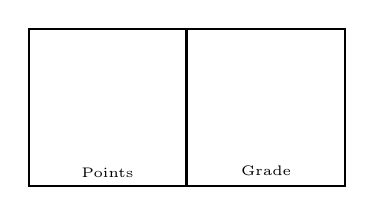
\begin{tikzpicture}[thick]
		\node (points) at (0,0) [draw,minimum size=2cm] {};
		\node (lbl-points) at (points.south) [anchor=south,font=\tiny] {Points};
		\node (grade) at (points.east) [draw,minimum size=2cm,anchor=west,
			outer sep=0] {};
		\node (lbl-grade) at (grade.south) [anchor=south,font=\tiny] {Grade};
	\end{tikzpicture}

	\begin{flushright}

		% Update this with your team number
		\huge\bfseries
		Team: XX \\[1em]

		% Update this with your matriculation number, first name, second name
		\large
		1326907 David FREISMUTH \\
	
	\end{flushright}

	\vspace{5em}

	\begin{center}
		{\huge Digital Integrated Circuits Lab (LDIS)}\\[1em]
		{\Large 384.088, Summer Term 2019} \\[2em]
		{\large Supervisors:\\[.5em]
			Christian Krieg, David Radakovits, Axel Jantsch} \\[10em]

		{\Huge Task 2:\\[.5em]Design Characterization,\\[.5em]Bus Communication}\\[10em]
	\end{center}


%	\begin{abstract}
%
%		Enter the abstract of your report here. An abstract summarizes your
%		entire work (i.e., problem statement, motivation, methodology, key
%		findings). It is a good strategy to write a first version of the abstract
%		when you start to work on your report. This gives you a good guideline
%		what to	put and what not to put into the report. Ideally, you re-write
%		the abstract once you finished your report, because only at this point
%		you have all the information available to create a good abstract.
%
%	\end{abstract}

\end{titlepage}
%
%----------------------------------------------------------------------------
%
\section{Characterize your design from Task 1}
\label{sec:characterization}

In order to make your design implementation comparable to other
implementations, simulate your design using Vivado and perform the
following measurements:

\begin{enumerate}

	\item{Timing analysis}

	\item{Power analysis}

	\item{Resource consumption}

\end{enumerate}

Create a design space vector for your design.%
The design space vector holds the following parameters, where $t_{max}$
is the maximum delay for the critical path, $P_{avg}$ is the average
power consumption for your design (vector-less post-place-and-route power
estimation), and $r$ is the percentage of resources used in your
implementation for the Nexys 4 DDR board (for sake of simplicity, use the
percentage of slices):

\begin{align}
	\vec{v} =
		\begin{bmatrix}
		t_{max}  \\
		P_{avg}\\
		r  \\
	\end{bmatrix}
\end{align}

You will find information on power estimation~\autocite{xpe} and timing
analysis~\autocite{timing} on the web.

Get the design space vectors of your colleagues, and visualize the
three-dimensional design space. Use black crosses for the vectors of your
colleagues, and a filled circle for your own vector.
%
%----------------------------------------------------------------------------
%
\section{Create an AMBA APB interface}

The goal of this subtask is to make your design accessible from other
\gls{ip} cores via the \gls{amba} \gls{apb}. Consult the \gls{apb}
specification~\autocite{apb}, and:

\begin{enumerate}

	\item{Implement a bus controller that implements the use case for your
		task}

	\item{Implement a bus interface for any sub-component of your design
		from Task~1 (sampling, data processing, output).}

	\item{Implement a module that takes the user input for runtime parameters
		and connect it to the bus}

\end{enumerate}

\begin{figure}[h!]
	\centering
	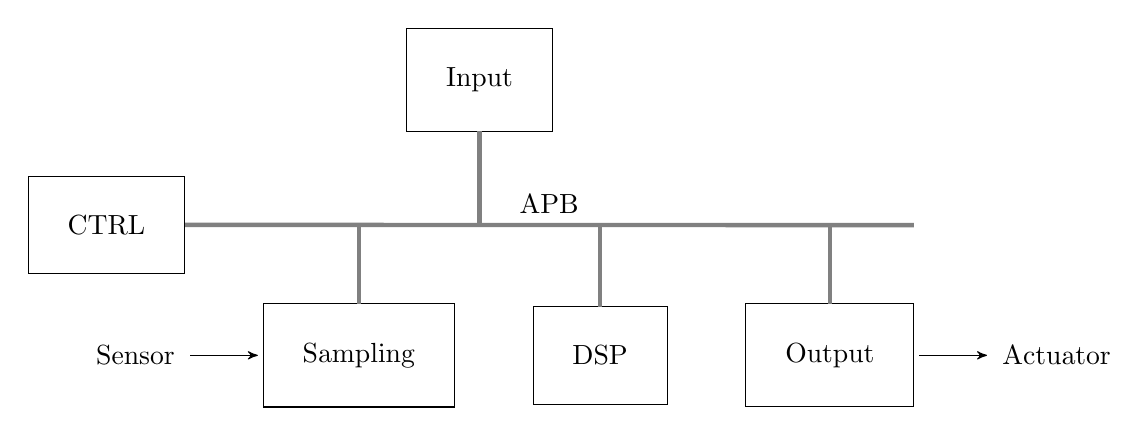
\begin{tikzpicture}[
	nd/.append style={draw, minimum height=1cm, inner sep=5mm, outer sep=0, align=center},
	ed/.style={->, >= stealth', shorten >=2pt, shorten <= 2pt},
]

	\node(input)[nd]{Sampling};
	\node(dsp)[nd, right=of input]{DSP};
	\node(output)[nd, right=of dsp]{Output};
	\node(userinput) at ($ (input)!.5!(dsp) +(0,3.5) $) [nd] {Input};

	\draw[ed,<-] (input.west) -- ++(-1cm,0) node[left]{Sensor};
%	\draw[ed] (input) -- (dsp);
%	\draw[ed] (dsp) -- (output);
	\draw[ed] (output.east) -- ++(1cm,0) node[right]{Actuator};

	\begin{scope}[ultra thick, gray]
		\draw ($ (input.north west) + (-1cm,1cm) $) coordinate(bus) -- node [above,midway,black] {APB} ($ (output.north east) +(0,1cm) $);
		\draw (input) -- (input |- bus);
		\draw (dsp) -- (dsp |- bus);
		\draw (output) -- (output |- bus);
		\draw (userinput) -- (userinput |- bus);
	\end{scope}

	\node (ctrl) at (bus) [nd,anchor=east]{CTRL};

\end{tikzpicture}
	\caption{System of Task~1 equipped with an \gls{apb}}
	\label{fig:audio-block}
\end{figure}

Your system should be able to take the user input, parametrize the system
according to the user input, and perform the actual task. Instead of
directly connecting each of the sub-components directly, the modules should
communicate over the \gls{apb}. The audio system can be treated as one
module; as it is kind of a real-time system, it wouldn't make a lot of sense
to let it communicate over the \gls{apb}. The user-input (e.g., cut-off
freuqency) should be set over the \gls{apb}.

\pagebreak
%------------------------------------------------------------------------------


\section{Design Characterization}
\label{sec:task1}
In this task, the metric introduced in \Cref{sec:characterization} shall be applied on the design, that has been established in the previous task. The values that are used to calculate the vector, can be found in Vivado. 

\subsection*{Critical Path Delay $t_{max}$}
After successful implementation, the delay of the critical path $t_{max}$ can be retrieved by executing the command \\ \lstinline[breaklines=true]{report_timing_summary} in the tcl console. The value \lstinline{DataPathDelay} describes the critical path delay.

\begin{figure}[h!]
	\centering
	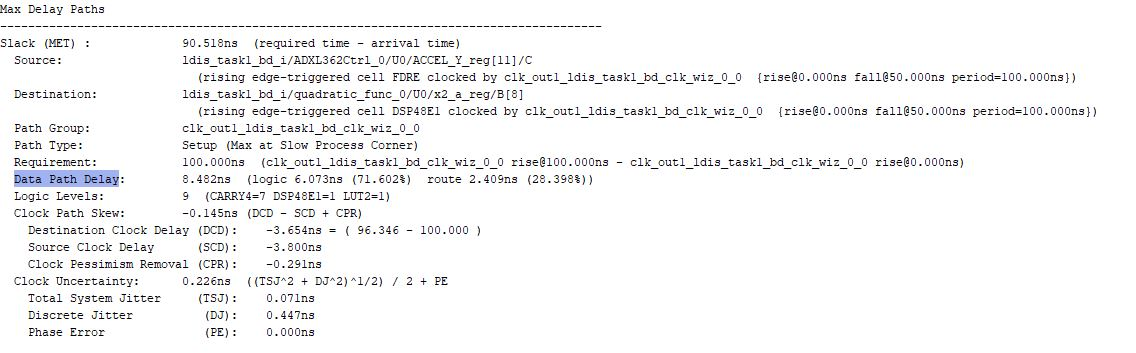
\includegraphics[width = \textwidth]{fig/dataPathDelay.jpg}
	\caption{tcl console output, after executing the command \lstinline{report_timing_summary}.}
	\label{fig:timingSummary}
\end{figure}

\subsection*{Average Power Consumption $P_{avg}$}
The average power consumption $P_{avg}$ can be seen in the project summary view. See \Cref{fig:pavg} for reference.

\begin{figure}[h!]
	\centering
	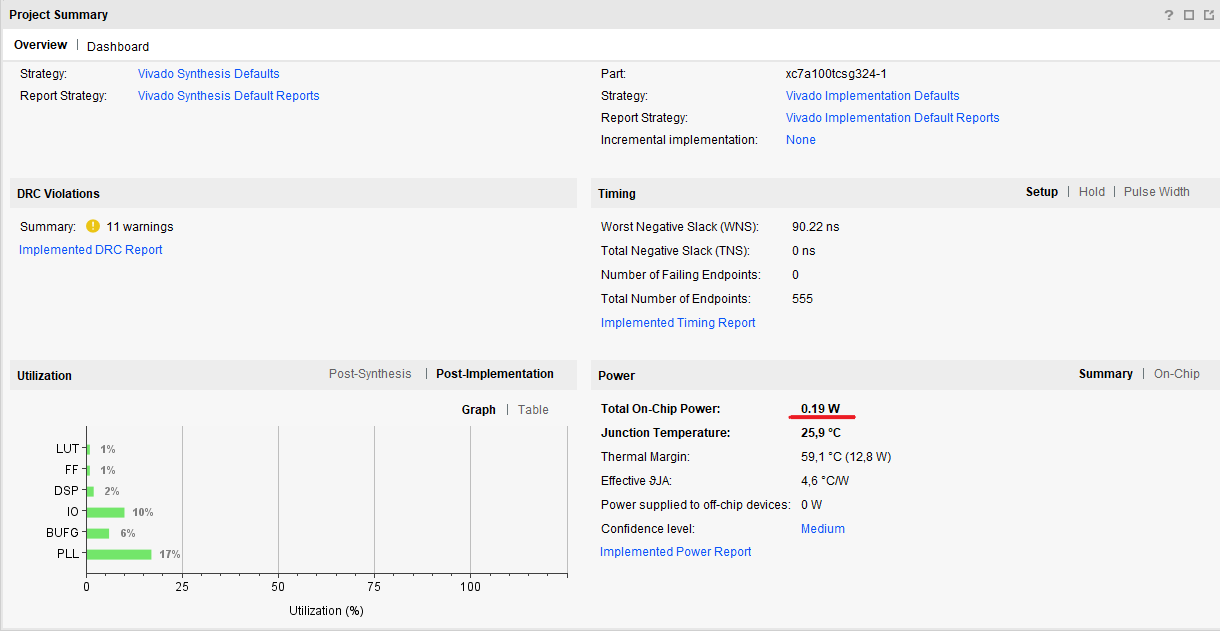
\includegraphics[width = \textwidth]{fig/Pavg.png}
	\caption{The project summary view of a Vivado project. The average power consumption value has been marked.}
	\label{fig:pavg}
\end{figure}

\subsection*{Resource Consumption $r$}
The resource consumption shall be measured by the usage of logical slices. It is calculated from the values retrieved by the tcl command\lstinline{report_utilization}. \Cref{math:util} shows the formula that is used to compute the resource consumption. 

\begin{figure}[h]
	\centering
	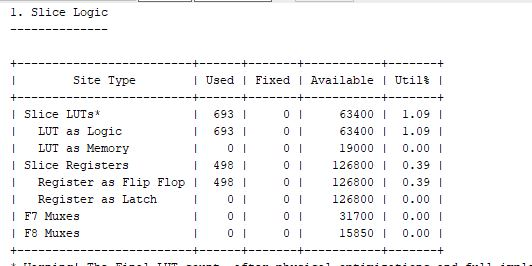
\includegraphics[width = \textwidth]{fig/resourceConsumption.jpg}
	\caption{tcl console output, after executing the command \lstinline{report_utilization}.}
	\label{fig:utilization}
\end{figure}

\begin{align}
        \frac{\textrm{Slice Luts used} + \textrm{Slice Registers used} + \textrm{F7 Muxes used} + \textrm{F8 Muxes used}}{\textrm{Slice Luts available} + \textrm{Slice Registers available} + \textrm{F7 Muxes available} + \textrm{F8 Muxes available}} \label{math:util}
\end{align}

\subsection*{Results}
By applying the metrics established in \Cref{sec:task1}, the vector in \Cref{math:vector} is yielded.


\begin{align}
	\vec{v} =
		\begin{bmatrix}
		t_{max}  \\
		P_{avg}\\
		r  \\
	\end{bmatrix}
	=
    \begin{bmatrix}
		8,896 ns  \\
		0,190 W\\
		0,005 	 \\
	\end{bmatrix} \label{math:vector}
\end{align}

The design space vectors of other solutions can be seen in \Cref{tab:results}. \Cref{fig:3dplot} visualizes those vectors.

\begin{figure}[h]
    \begin{center}
        \begin{tabular}{ r r r }
        \hline\hline
        $t_{max}$ [ns] & $P_{avg}$ [W] & $r$ [\%] \\
        \hline\hline
            8,896   & 0,190  & 0,005  \\
            2,000   & 0,111  & 0,150  \\
            3,000   & 0,207  & 1,000  \\
        \hline\hline 
        \end{tabular}
    \end{center}
    \label{tab:results}
    \caption{Design space vector of other solutions.}
\end{figure}



\begin{figure}[h!]
 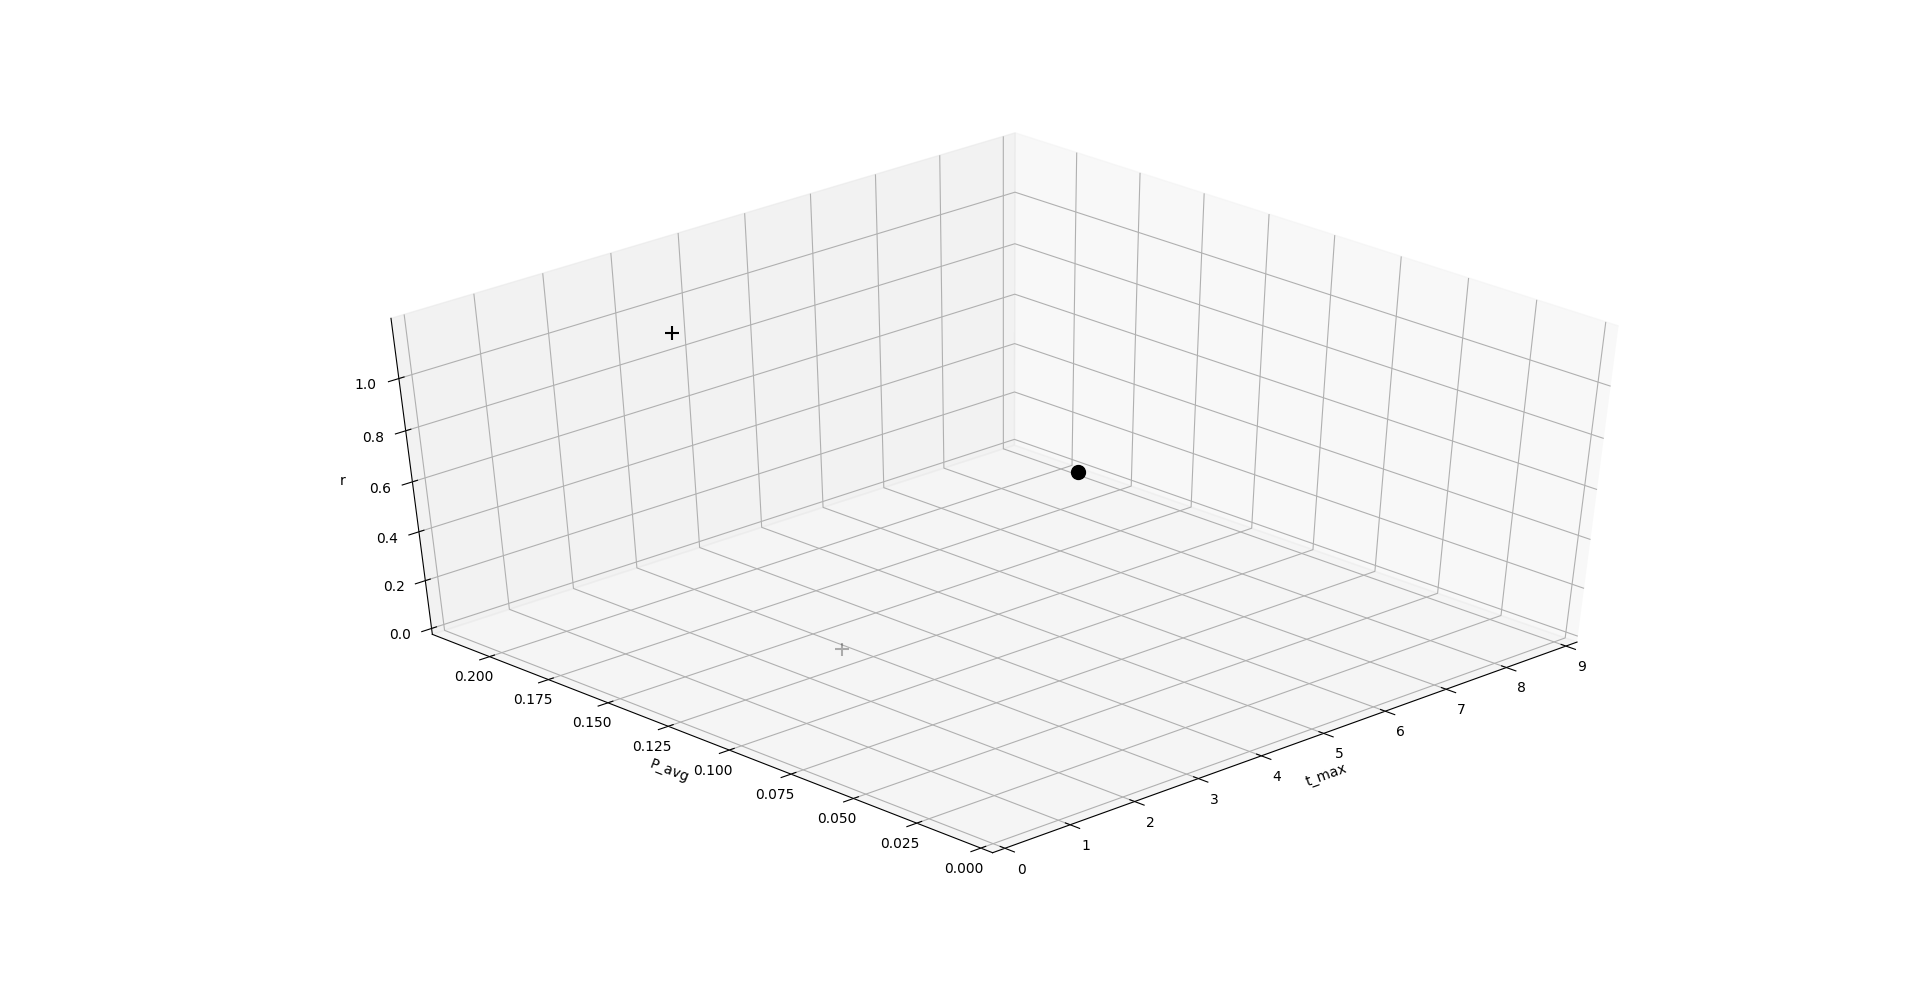
\includegraphics[width = \textwidth]{fig/3dplot.png}
 \caption{The plot of all design space vectors. Crosses mark the vectors of other designs. The circle marks the vector of the design that has been established during the course of this task.}
 \label{fig:3dplot}
\end{figure}


\section{APB Implementation}
In this task, the design from task 1 shall be extended with an APB bus, to enable  a modular access to the design sub components, as seen in \Cref{fig:audio-block}. \\
To achieve this modularity, a slave interface and a bus controller has been designed. The following sections describe the details of the implementation.

\subsection{Slave Interface}
The slave interface incorporates all necessary ports to be conform to the APB specification ( \lstinline[breaklines = true]{PWDATA, PADDR, PWRITE, PSEL, PENABLE, PRDATA, PREADY}). To be able to connect to the sub components that have been designed in the previous task, the proprietary \textit{REG} interface \lstinline[breaklines = true]{REG_IN, REG_OUT, REG_RW, REG_WREN, REG_ADDR, RED_RDY} is exposed. Furthermore, the interface contains a parameterizable count of 32 bit registers, which are addressable via APB and REG interface. 

\begin{minipage}{\linewidth}
\begin{lstlisting}[
language = VHDL,
label = {lst:SlaveIf},
caption = {Port of the APB Slave Interface}]
 entity APBSlaveIF is
    Generic(
        pindex     : integer := 0;
        regCount   : integer := 4;
        slaveCount : integer := 2
    );
    Port (
        CLK : in STD_LOGIC;
        
        --APB Slave Interface
        PWDATA  : in  STD_LOGIC_VECTOR (31 downto 0);
        PADDR   : in  STD_LOGIC_VECTOR (31 downto 0);
        PWRITE  : in  STD_LOGIC;
        PSEL    : in  STD_LOGIC_VECTOR (slaveCount-1 downto 0);
        PENABLE : in  STD_LOGIC;
        PRDATA  : out STD_LOGIC_VECTOR (31 downto 0) := x"00000000";
        PREADY  : out STD_LOGIC;
        
        --Interface for attached module
        REG_IN   : in STD_LOGIC_VECTOR (31 downto 0);
        REG_OUT  : out STD_LOGIC_VECTOR (31 downto 0) := x"00000000";
        REG_RW   : in STD_LOGIC;  -- High enables REG read, Low enables REG write
        REG_WREN : in STD_LOGIC;  -- Asserts REG write or read action
        REG_ADDR : in STD_LOGIC_VECTOR( 
            INTEGER(CEIL(LOG2(REAL(regCount))))+1 downto 0);  -- Asserts REG write or read action
        REG_RDY  : out STD_LOGIC -- Is set to high, if a transaction has been finished.
    );    
end APBSlaveIF;
\end{lstlisting}
\end{minipage}

The state machine diagram of the REG interface can be seen in \Cref{fig:RegStateMachine}.

\begin{figure}[h!]
 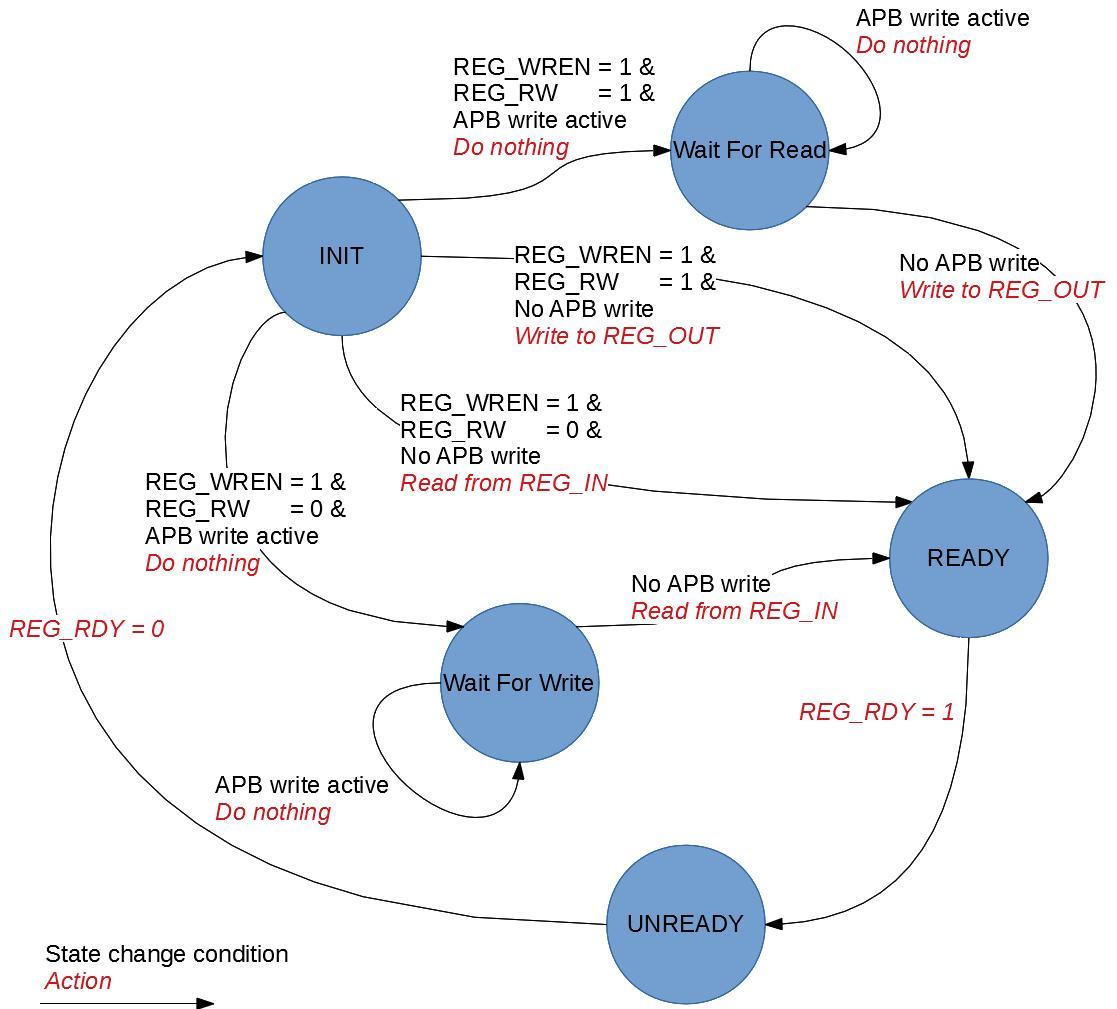
\includegraphics[width = \textwidth]{fig/REGStateMachine.jpg}
 \caption{The state machine diagram of the REG interface.}
 \label{fig:RegStateMachine}
\end{figure}


\subsection{Bus Controller}
The bus controller is responsible for controlling the data flow to and from the APB slaves. The port declaration can be seen in \Cref{lst:MasterIf}. The state machine of the bus controller is illustrated in \Cref{fig:stateMachineMaster}.

\begin{minipage}{\linewidth}
\begin{lstlisting}[
language = VHDL,
label = {lst:MasterIf},
caption = {Port of the APB Bus Master}]
entity CTRLWrapper is
    Generic(
        slaveCount : INTEGER := 4
    ); 
    Port ( 
        CLK : in STD_LOGIC;     
        --APB Slave Interface
        PWDATA     : out  STD_LOGIC_VECTOR (31 downto 0);
        PADDR      : out  STD_LOGIC_VECTOR (31 downto 0);
        PWRITE     : out  STD_LOGIC;
        PSEL       : out  STD_LOGIC_VECTOR (slaveCount-1 downto 0);
        PENABLE    : out  STD_LOGIC;
        PRDATA_S1  : in   STD_LOGIC_VECTOR (31 downto 0) := x"00000000";
        PRDATA_S2  : in   STD_LOGIC_VECTOR (31 downto 0) := x"00000000";
        PRDATA_S3  : in   STD_LOGIC_VECTOR (31 downto 0) := x"00000000";
        PRDATA_S4  : in   STD_LOGIC_VECTOR (31 downto 0) := x"00000000";
        PREADY_S1  : in   STD_LOGIC;        
        PREADY_S2  : in   STD_LOGIC;   
        PREADY_S3  : in   STD_LOGIC;
        PREADY_S4  : in   STD_LOGIC;
                      
        DEBUG_ACC_VAL  : out   STD_LOGIC_VECTOR (31 downto 0);
        DEBUG_DSP_VAL  : out   STD_LOGIC_VECTOR (31 downto 0)
    );
end CTRLWrapper;
\end{lstlisting}
\end{minipage}

\begin{figure}[h!]
 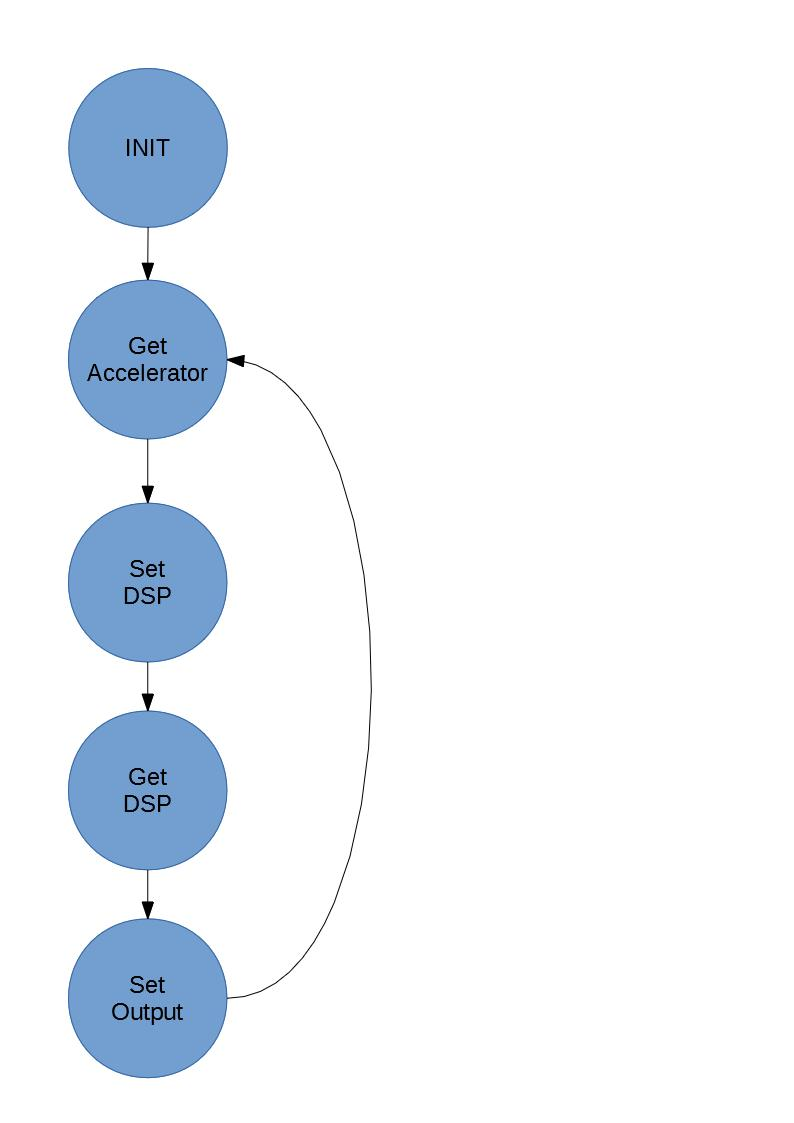
\includegraphics[width = \textwidth]{fig/MasterStatemachine.jpg}
 \caption{The state machine diagram describing the behavior of the APB bus master.}
 \label{fig:stateMachineMaster}
\end{figure}


%
%----------------------------------------------------------------------------
%
\end{document}
%
%----------------------------------------------------------------------------
